\documentclass[aspectratio=169,11pt]{beamer}
% =====================================================================
%  pds-beamer.tex — Estilo común de las transparencias.
%
%  Uso (desde teoría/Tx/transparencias/):
%     \documentclass[aspectratio=169,11pt]{beamer}
%     % =====================================================================
%  pds-beamer.tex — Estilo común de las transparencias.
%
%  Uso (desde teoría/Tx/transparencias/):
%     \documentclass[aspectratio=169,11pt]{beamer}
%     % =====================================================================
%  pds-beamer.tex — Estilo común de las transparencias.
%
%  Uso (desde teoría/Tx/transparencias/):
%     \documentclass[aspectratio=169,11pt]{beamer}
%     \input{../../comun/pds-beamer}
%     \title{...}  \subtitle{Tema x · ...}
%     \begin{document}
%       \portada
%       ...
%     \end{document}
%  Compilar con:  latexmk -xelatex  (o «make» desde teoría/)
% =====================================================================

\usetheme{Boadilla}
\usecolortheme{orchid}
\usefonttheme{professionalfonts}
\setbeamercovered{transparent}
\setbeamersize{text margin left=0.8cm, text margin right=0.8cm}
\setbeamertemplate{navigation symbols}{}
\setbeamertemplate{itemize item}[square]
\setbeamertemplate{itemize subitem}[circle]
\setbeamertemplate{itemize subsubitem}[triangle]
\setbeamertemplate{enumerate item}[square]
\setbeamertemplate{enumerate subitem}[circle]
\setbeamertemplate{caption}{\raggedright\insertcaption\par}

\input{../../comun/pds-comun.tex}

% Tipografía: Fira Sans + Fira Math (legibles en proyector)
\usepackage{fontspec}
\usepackage{unicode-math}
% Se cargan por nombre de fichero para que funcionen con cualquier
% instalación de TeX Live (o MiKTeX) sin instalar fuentes en el sistema.
\setmainfont{FiraSans}[Extension=.otf, UprightFont=*-Regular, BoldFont=*-SemiBold,
  ItalicFont=*-Italic, BoldItalicFont=*-SemiBoldItalic]
\setsansfont{FiraSans}[Extension=.otf, UprightFont=*-Regular, BoldFont=*-SemiBold,
  ItalicFont=*-Italic, BoldItalicFont=*-SemiBoldItalic]
\setmonofont{FiraMono}[Extension=.otf, UprightFont=*-Regular, BoldFont=*-Medium, AutoFakeSlant=0.15, Scale=0.92]
\setmathfont{FiraMath-Regular.otf}
\setmathfont{latinmodern-math.otf}[range={"229B,"22EE,"22F1}]

% Colores del tema ajustados a la paleta común (más contraste)
\setbeamercolor{structure}{fg=pdsazul}
\setbeamercolor{alerted text}{fg=pdsrojo}
\setbeamercolor{example text}{fg=pdsverde}
\setbeamercolor{block title}{bg=pdsazul, fg=white}
\setbeamercolor{block body}{bg=pdsfondo}
\setbeamercolor{block title alerted}{bg=pdsrojo, fg=white}
\setbeamercolor{block body alerted}{bg=pdsrojo!6}
\setbeamercolor{block title example}{bg=pdsverde, fg=white}
\setbeamercolor{block body example}{bg=pdsverde!6}
\setbeamercolor{frametitle}{fg=pdsazul, bg=white}
\setbeamerfont{frametitle}{size=\large, series=\bfseries}
\setbeamerfont{block title}{size=\normalsize, series=\bfseries}
\setbeamertemplate{blocks}[rounded][shadow=false]

% Logo en la esquina superior derecha de cada transparencia
\pgfdeclareimage[height=0.8cm]{logo}{../../comun/ucm.png}
\addtobeamertemplate{frametitle}{}{%
  \begin{tikzpicture}[remember picture, overlay]
    \node[anchor=north east, inner sep=0pt] at ([xshift=-0.25cm, yshift=-0.2cm]current page.north east) {\pgfuseimage{logo}};
  \end{tikzpicture}}

% Datos de portada
\author[\autorescorto]{\autores}
\institute[UCM]{\footnotesize\departamento\\\universidad}
\date[\curso]{\footnotesize\grado\\\curso}

\newcommand{\portada}{%
  \begin{frame}[plain]
    \begin{center}
      
\includegraphics[height=1.9cm]{../../comun/ucm.png}
    \end{center}
    \vspace{-0.4cm}
    \titlepage
  \end{frame}}

% Índice al empezar cada sección
\AtBeginSection[]{%
  \begin{frame}{Contenido}
    \tableofcontents[currentsection, hideothersubsections]
  \end{frame}}

\renewcommand{\pdscodesize}{\scriptsize}

% Utilidades
% \herramienta{T1-convolucion-continua}: enlace a la página publicada de
% herramientas/html (se abre en el navegador, sin instalar nada).
% \herramientaservidor{server/....py}: app que necesita Python (bokeh serve).
\newcommand{\urlherramientas}{https://ucm-237.github.io/PdS/}
\newcommand{\herramienta}[1]{%
  \par\vfill\hfill{\scriptsize\color{pdsgris}\faIcon\ \href{\urlherramientas#1.html}{Herramienta interactiva: \texttt{#1}}}}
\newcommand{\herramientaservidor}[1]{%
  \par\vfill\hfill{\scriptsize\color{pdsgris}\faIcon\ Herramienta interactiva (con Python): \texttt{herramientas/#1}}}
\newcommand{\faIcon}{\textbf{▶}}
\newcommand{\gris}[1]{{\color{pdsgris}#1}}
\newcommand{\nota}[1]{\par\vspace{2pt}{\footnotesize\color{pdsgris}\textit{#1}}\par}
% Nota sobre una errata de versiones anteriores (solo con \ERRATAS)
\newcommand{\errata}[1]{\iferratas\nota{Errata de versiones anteriores: #1}\fi}
\newcommand{\apuntes}[1]{\nota{Más detalle en los apuntes, #1.}}

% Bloques con nombre en castellano
\newenvironment{definicion}[1][Definición]{\begin{block}{#1}}{\end{block}}
\newenvironment{importante}[1][Importante]{\begin{alertblock}{#1}}{\end{alertblock}}
\newenvironment{ejemplo}[1][Ejemplo]{\begin{exampleblock}{#1}}{\end{exampleblock}}

%     \title{...}  \subtitle{Tema x · ...}
%     \begin{document}
%       \portada
%       ...
%     \end{document}
%  Compilar con:  latexmk -xelatex  (o «make» desde teoría/)
% =====================================================================

\usetheme{Boadilla}
\usecolortheme{orchid}
\usefonttheme{professionalfonts}
\setbeamercovered{transparent}
\setbeamersize{text margin left=0.8cm, text margin right=0.8cm}
\setbeamertemplate{navigation symbols}{}
\setbeamertemplate{itemize item}[square]
\setbeamertemplate{itemize subitem}[circle]
\setbeamertemplate{itemize subsubitem}[triangle]
\setbeamertemplate{enumerate item}[square]
\setbeamertemplate{enumerate subitem}[circle]
\setbeamertemplate{caption}{\raggedright\insertcaption\par}

% =====================================================================
%  pds-comun.tex — Paquetes, colores y estilos de código comunes a
%  transparencias, apuntes y hojas de ejercicios. Compilar con XeLaTeX.
%  No cargar directamente: lo cargan pds-beamer.tex y pds-apuntes.tex.
% =====================================================================

\usepackage{polyglossia}
\setmainlanguage{spanish}
\usepackage{mathtools}
\usepackage{graphicx}
\usepackage{booktabs}
\usepackage{multirow}
\usepackage{array}
\usepackage{xcolor}
\usepackage{tikz}
\usetikzlibrary{positioning,arrows.meta,calc,shapes.geometric,decorations.pathreplacing}
\usepackage{listings}
\usepackage{siunitx}
\sisetup{output-decimal-marker={,}, group-separator={\,}, per-mode=symbol}

% Notas de erratas de versiones anteriores: no se imprimen salvo que se
% defina \ERRATAS antes de cargar el estilo (make ERRATAS=1)
\newif\iferratas
\ifdefined\ERRATAS \erratastrue \fi

% Ruta común (logo y figuras compartidas)
\providecommand{\rutacomun}{../../comun/}
\input{\rutacomun datos.tex}

% ---------------------------------------------------------------------
%  Paleta (la misma que usan las figuras generadas con Python,
%  ver comun/pds_estilo.py)
% ---------------------------------------------------------------------
\definecolor{pdsazul}{HTML}{2B3A8C}
\definecolor{pdsrojo}{HTML}{C0392B}
\definecolor{pdsverde}{HTML}{1E7B4F}
\definecolor{pdsnaranja}{HTML}{D9822B}
\definecolor{pdsgris}{HTML}{5A5A66}
\definecolor{pdsfondo}{HTML}{F3F4FA}
\definecolor{pdscodigo}{HTML}{F7F7F2}

% ---------------------------------------------------------------------
%  Diagramas de bloques (TikZ)
% ---------------------------------------------------------------------
\tikzset{
  bloque/.style={rectangle, rounded corners=2pt, draw=pdsazul!80, fill=pdsfondo,
                 very thick, minimum height=8mm, minimum width=14mm, align=center},
  sumador/.style={circle, draw=pdsazul!80, fill=pdsfondo, thick, inner sep=1.5pt},
  flecha/.style={-{Stealth[length=2.2mm]}, thick, pdsgris},
}

% ---------------------------------------------------------------------
%  Código: Python y Matlab en paralelo
% ---------------------------------------------------------------------
\newcommand{\pdscodesize}{\footnotesize}
\lstdefinestyle{pds}{
  basicstyle=\ttfamily\pdscodesize,
  keywordstyle=\color{pdsazul}\bfseries,
  commentstyle=\color{pdsverde}\itshape,
  stringstyle=\color{pdsrojo},
  numbers=none,
  backgroundcolor=\color{pdscodigo},
  frame=single, rulecolor=\color{pdsgris!40}, framerule=0.4pt,
  xleftmargin=2pt, xrightmargin=2pt, aboveskip=2pt, belowskip=2pt,
  columns=fullflexible, keepspaces=true,
  showstringspaces=false, breaklines=true, tabsize=4,
  upquote=true,
  % Con XeLaTeX, listings desordena los caracteres no ASCII junto a
  % dígitos («2π» sale «π2»): se sustituyen por su versión matemática.
  literate={π}{{$\pi$}}1 {δ}{{$\delta$}}1 {ω}{{$\omega$}}1 {Ω}{{$\Omega$}}1
           {≈}{{$\approx$}}1 {µ}{{$\mu$}}1 {·}{{$\cdot$}}1 {α}{{$\alpha$}}1
           {á}{{á}}1 {é}{{é}}1 {í}{{í}}1 {ó}{{ó}}1 {ú}{{ú}}1 {ñ}{{ñ}}1 {¿}{{¿}}1,
}
\lstdefinestyle{python}{style=pds, language=Python,
  morekeywords={as,True,False,None}}
\lstdefinestyle{matlab}{style=pds, language=Matlab,
  morekeywords={function,end,true,false}}

% \codigo{<ruta sin extensión>} muestra el mismo ejemplo en Python
% y en Matlab, uno al lado del otro. Los ficheros viven en
% ../codigo/python/<nombre>.py y ../codigo/matlab/<nombre>.m y se
% ejecutan en las pruebas (make prueba-codigo).
\newcommand{\rutacodigo}{../codigo/}
\newcommand{\codigoetiqueta}[1]{{\sffamily\scriptsize\bfseries\color{pdsgris}#1}}
\newcommand{\codigo}[2][]{%
  \par\noindent
  \begin{minipage}[t]{0.495\linewidth}
    \codigoetiqueta{Python}\par\vspace{1pt}
    \lstinputlisting[style=python,#1]{\rutacodigo python/#2.py}
  \end{minipage}\hfill
  \begin{minipage}[t]{0.495\linewidth}
    \codigoetiqueta{Matlab}\par\vspace{1pt}
    \lstinputlisting[style=matlab,#1]{\rutacodigo matlab/#2.m}
  \end{minipage}\par}

\input{\rutacomun notacion.tex}


% Tipografía: Fira Sans + Fira Math (legibles en proyector)
\usepackage{fontspec}
\usepackage{unicode-math}
% Se cargan por nombre de fichero para que funcionen con cualquier
% instalación de TeX Live (o MiKTeX) sin instalar fuentes en el sistema.
\setmainfont{FiraSans}[Extension=.otf, UprightFont=*-Regular, BoldFont=*-SemiBold,
  ItalicFont=*-Italic, BoldItalicFont=*-SemiBoldItalic]
\setsansfont{FiraSans}[Extension=.otf, UprightFont=*-Regular, BoldFont=*-SemiBold,
  ItalicFont=*-Italic, BoldItalicFont=*-SemiBoldItalic]
\setmonofont{FiraMono}[Extension=.otf, UprightFont=*-Regular, BoldFont=*-Medium, AutoFakeSlant=0.15, Scale=0.92]
\setmathfont{FiraMath-Regular.otf}
\setmathfont{latinmodern-math.otf}[range={"229B,"22EE,"22F1}]

% Colores del tema ajustados a la paleta común (más contraste)
\setbeamercolor{structure}{fg=pdsazul}
\setbeamercolor{alerted text}{fg=pdsrojo}
\setbeamercolor{example text}{fg=pdsverde}
\setbeamercolor{block title}{bg=pdsazul, fg=white}
\setbeamercolor{block body}{bg=pdsfondo}
\setbeamercolor{block title alerted}{bg=pdsrojo, fg=white}
\setbeamercolor{block body alerted}{bg=pdsrojo!6}
\setbeamercolor{block title example}{bg=pdsverde, fg=white}
\setbeamercolor{block body example}{bg=pdsverde!6}
\setbeamercolor{frametitle}{fg=pdsazul, bg=white}
\setbeamerfont{frametitle}{size=\large, series=\bfseries}
\setbeamerfont{block title}{size=\normalsize, series=\bfseries}
\setbeamertemplate{blocks}[rounded][shadow=false]

% Logo en la esquina superior derecha de cada transparencia
\pgfdeclareimage[height=0.8cm]{logo}{../../comun/ucm.png}
\addtobeamertemplate{frametitle}{}{%
  \begin{tikzpicture}[remember picture, overlay]
    \node[anchor=north east, inner sep=0pt] at ([xshift=-0.25cm, yshift=-0.2cm]current page.north east) {\pgfuseimage{logo}};
  \end{tikzpicture}}

% Datos de portada
\author[\autorescorto]{\autores}
\institute[UCM]{\footnotesize\departamento\\\universidad}
\date[\curso]{\footnotesize\grado\\\curso}

\newcommand{\portada}{%
  \begin{frame}[plain]
    \begin{center}
      
\includegraphics[height=1.9cm]{../../comun/ucm.png}
    \end{center}
    \vspace{-0.4cm}
    \titlepage
  \end{frame}}

% Índice al empezar cada sección
\AtBeginSection[]{%
  \begin{frame}{Contenido}
    \tableofcontents[currentsection, hideothersubsections]
  \end{frame}}

\renewcommand{\pdscodesize}{\scriptsize}

% Utilidades
% \herramienta{T1-convolucion-continua}: enlace a la página publicada de
% herramientas/html (se abre en el navegador, sin instalar nada).
% \herramientaservidor{server/....py}: app que necesita Python (bokeh serve).
\newcommand{\urlherramientas}{https://ucm-237.github.io/PdS/}
\newcommand{\herramienta}[1]{%
  \par\vfill\hfill{\scriptsize\color{pdsgris}\faIcon\ \href{\urlherramientas#1.html}{Herramienta interactiva: \texttt{#1}}}}
\newcommand{\herramientaservidor}[1]{%
  \par\vfill\hfill{\scriptsize\color{pdsgris}\faIcon\ Herramienta interactiva (con Python): \texttt{herramientas/#1}}}
\newcommand{\faIcon}{\textbf{▶}}
\newcommand{\gris}[1]{{\color{pdsgris}#1}}
\newcommand{\nota}[1]{\par\vspace{2pt}{\footnotesize\color{pdsgris}\textit{#1}}\par}
% Nota sobre una errata de versiones anteriores (solo con \ERRATAS)
\newcommand{\errata}[1]{\iferratas\nota{Errata de versiones anteriores: #1}\fi}
\newcommand{\apuntes}[1]{\nota{Más detalle en los apuntes, #1.}}

% Bloques con nombre en castellano
\newenvironment{definicion}[1][Definición]{\begin{block}{#1}}{\end{block}}
\newenvironment{importante}[1][Importante]{\begin{alertblock}{#1}}{\end{alertblock}}
\newenvironment{ejemplo}[1][Ejemplo]{\begin{exampleblock}{#1}}{\end{exampleblock}}

%     \title{...}  \subtitle{Tema x · ...}
%     \begin{document}
%       \portada
%       ...
%     \end{document}
%  Compilar con:  latexmk -xelatex  (o «make» desde teoría/)
% =====================================================================

\usetheme{Boadilla}
\usecolortheme{orchid}
\usefonttheme{professionalfonts}
\setbeamercovered{transparent}
\setbeamersize{text margin left=0.8cm, text margin right=0.8cm}
\setbeamertemplate{navigation symbols}{}
\setbeamertemplate{itemize item}[square]
\setbeamertemplate{itemize subitem}[circle]
\setbeamertemplate{itemize subsubitem}[triangle]
\setbeamertemplate{enumerate item}[square]
\setbeamertemplate{enumerate subitem}[circle]
\setbeamertemplate{caption}{\raggedright\insertcaption\par}

% =====================================================================
%  pds-comun.tex — Paquetes, colores y estilos de código comunes a
%  transparencias, apuntes y hojas de ejercicios. Compilar con XeLaTeX.
%  No cargar directamente: lo cargan pds-beamer.tex y pds-apuntes.tex.
% =====================================================================

\usepackage{polyglossia}
\setmainlanguage{spanish}
\usepackage{mathtools}
\usepackage{graphicx}
\usepackage{booktabs}
\usepackage{multirow}
\usepackage{array}
\usepackage{xcolor}
\usepackage{tikz}
\usetikzlibrary{positioning,arrows.meta,calc,shapes.geometric,decorations.pathreplacing}
\usepackage{listings}
\usepackage{siunitx}
\sisetup{output-decimal-marker={,}, group-separator={\,}, per-mode=symbol}

% Notas de erratas de versiones anteriores: no se imprimen salvo que se
% defina \ERRATAS antes de cargar el estilo (make ERRATAS=1)
\newif\iferratas
\ifdefined\ERRATAS \erratastrue \fi

% Ruta común (logo y figuras compartidas)
\providecommand{\rutacomun}{../../comun/}
\input{\rutacomun datos.tex}

% ---------------------------------------------------------------------
%  Paleta (la misma que usan las figuras generadas con Python,
%  ver comun/pds_estilo.py)
% ---------------------------------------------------------------------
\definecolor{pdsazul}{HTML}{2B3A8C}
\definecolor{pdsrojo}{HTML}{C0392B}
\definecolor{pdsverde}{HTML}{1E7B4F}
\definecolor{pdsnaranja}{HTML}{D9822B}
\definecolor{pdsgris}{HTML}{5A5A66}
\definecolor{pdsfondo}{HTML}{F3F4FA}
\definecolor{pdscodigo}{HTML}{F7F7F2}

% ---------------------------------------------------------------------
%  Diagramas de bloques (TikZ)
% ---------------------------------------------------------------------
\tikzset{
  bloque/.style={rectangle, rounded corners=2pt, draw=pdsazul!80, fill=pdsfondo,
                 very thick, minimum height=8mm, minimum width=14mm, align=center},
  sumador/.style={circle, draw=pdsazul!80, fill=pdsfondo, thick, inner sep=1.5pt},
  flecha/.style={-{Stealth[length=2.2mm]}, thick, pdsgris},
}

% ---------------------------------------------------------------------
%  Código: Python y Matlab en paralelo
% ---------------------------------------------------------------------
\newcommand{\pdscodesize}{\footnotesize}
\lstdefinestyle{pds}{
  basicstyle=\ttfamily\pdscodesize,
  keywordstyle=\color{pdsazul}\bfseries,
  commentstyle=\color{pdsverde}\itshape,
  stringstyle=\color{pdsrojo},
  numbers=none,
  backgroundcolor=\color{pdscodigo},
  frame=single, rulecolor=\color{pdsgris!40}, framerule=0.4pt,
  xleftmargin=2pt, xrightmargin=2pt, aboveskip=2pt, belowskip=2pt,
  columns=fullflexible, keepspaces=true,
  showstringspaces=false, breaklines=true, tabsize=4,
  upquote=true,
  % Con XeLaTeX, listings desordena los caracteres no ASCII junto a
  % dígitos («2π» sale «π2»): se sustituyen por su versión matemática.
  literate={π}{{$\pi$}}1 {δ}{{$\delta$}}1 {ω}{{$\omega$}}1 {Ω}{{$\Omega$}}1
           {≈}{{$\approx$}}1 {µ}{{$\mu$}}1 {·}{{$\cdot$}}1 {α}{{$\alpha$}}1
           {á}{{á}}1 {é}{{é}}1 {í}{{í}}1 {ó}{{ó}}1 {ú}{{ú}}1 {ñ}{{ñ}}1 {¿}{{¿}}1,
}
\lstdefinestyle{python}{style=pds, language=Python,
  morekeywords={as,True,False,None}}
\lstdefinestyle{matlab}{style=pds, language=Matlab,
  morekeywords={function,end,true,false}}

% \codigo{<ruta sin extensión>} muestra el mismo ejemplo en Python
% y en Matlab, uno al lado del otro. Los ficheros viven en
% ../codigo/python/<nombre>.py y ../codigo/matlab/<nombre>.m y se
% ejecutan en las pruebas (make prueba-codigo).
\newcommand{\rutacodigo}{../codigo/}
\newcommand{\codigoetiqueta}[1]{{\sffamily\scriptsize\bfseries\color{pdsgris}#1}}
\newcommand{\codigo}[2][]{%
  \par\noindent
  \begin{minipage}[t]{0.495\linewidth}
    \codigoetiqueta{Python}\par\vspace{1pt}
    \lstinputlisting[style=python,#1]{\rutacodigo python/#2.py}
  \end{minipage}\hfill
  \begin{minipage}[t]{0.495\linewidth}
    \codigoetiqueta{Matlab}\par\vspace{1pt}
    \lstinputlisting[style=matlab,#1]{\rutacodigo matlab/#2.m}
  \end{minipage}\par}

\input{\rutacomun notacion.tex}


% Tipografía: Fira Sans + Fira Math (legibles en proyector)
\usepackage{fontspec}
\usepackage{unicode-math}
% Se cargan por nombre de fichero para que funcionen con cualquier
% instalación de TeX Live (o MiKTeX) sin instalar fuentes en el sistema.
\setmainfont{FiraSans}[Extension=.otf, UprightFont=*-Regular, BoldFont=*-SemiBold,
  ItalicFont=*-Italic, BoldItalicFont=*-SemiBoldItalic]
\setsansfont{FiraSans}[Extension=.otf, UprightFont=*-Regular, BoldFont=*-SemiBold,
  ItalicFont=*-Italic, BoldItalicFont=*-SemiBoldItalic]
\setmonofont{FiraMono}[Extension=.otf, UprightFont=*-Regular, BoldFont=*-Medium, AutoFakeSlant=0.15, Scale=0.92]
\setmathfont{FiraMath-Regular.otf}
\setmathfont{latinmodern-math.otf}[range={"229B,"22EE,"22F1}]

% Colores del tema ajustados a la paleta común (más contraste)
\setbeamercolor{structure}{fg=pdsazul}
\setbeamercolor{alerted text}{fg=pdsrojo}
\setbeamercolor{example text}{fg=pdsverde}
\setbeamercolor{block title}{bg=pdsazul, fg=white}
\setbeamercolor{block body}{bg=pdsfondo}
\setbeamercolor{block title alerted}{bg=pdsrojo, fg=white}
\setbeamercolor{block body alerted}{bg=pdsrojo!6}
\setbeamercolor{block title example}{bg=pdsverde, fg=white}
\setbeamercolor{block body example}{bg=pdsverde!6}
\setbeamercolor{frametitle}{fg=pdsazul, bg=white}
\setbeamerfont{frametitle}{size=\large, series=\bfseries}
\setbeamerfont{block title}{size=\normalsize, series=\bfseries}
\setbeamertemplate{blocks}[rounded][shadow=false]

% Logo en la esquina superior derecha de cada transparencia
\pgfdeclareimage[height=0.8cm]{logo}{../../comun/ucm.png}
\addtobeamertemplate{frametitle}{}{%
  \begin{tikzpicture}[remember picture, overlay]
    \node[anchor=north east, inner sep=0pt] at ([xshift=-0.25cm, yshift=-0.2cm]current page.north east) {\pgfuseimage{logo}};
  \end{tikzpicture}}

% Datos de portada
\author[\autorescorto]{\autores}
\institute[UCM]{\footnotesize\departamento\\\universidad}
\date[\curso]{\footnotesize\grado\\\curso}

\newcommand{\portada}{%
  \begin{frame}[plain]
    \begin{center}
      
\includegraphics[height=1.9cm]{../../comun/ucm.png}
    \end{center}
    \vspace{-0.4cm}
    \titlepage
  \end{frame}}

% Índice al empezar cada sección
\AtBeginSection[]{%
  \begin{frame}{Contenido}
    \tableofcontents[currentsection, hideothersubsections]
  \end{frame}}

\renewcommand{\pdscodesize}{\scriptsize}

% Utilidades
% \herramienta{T1-convolucion-continua}: enlace a la página publicada de
% herramientas/html (se abre en el navegador, sin instalar nada).
% \herramientaservidor{server/....py}: app que necesita Python (bokeh serve).
\newcommand{\urlherramientas}{https://ucm-237.github.io/PdS/}
\newcommand{\herramienta}[1]{%
  \par\vfill\hfill{\scriptsize\color{pdsgris}\faIcon\ \href{\urlherramientas#1.html}{Herramienta interactiva: \texttt{#1}}}}
\newcommand{\herramientaservidor}[1]{%
  \par\vfill\hfill{\scriptsize\color{pdsgris}\faIcon\ Herramienta interactiva (con Python): \texttt{herramientas/#1}}}
\newcommand{\faIcon}{\textbf{▶}}
\newcommand{\gris}[1]{{\color{pdsgris}#1}}
\newcommand{\nota}[1]{\par\vspace{2pt}{\footnotesize\color{pdsgris}\textit{#1}}\par}
% Nota sobre una errata de versiones anteriores (solo con \ERRATAS)
\newcommand{\errata}[1]{\iferratas\nota{Errata de versiones anteriores: #1}\fi}
\newcommand{\apuntes}[1]{\nota{Más detalle en los apuntes, #1.}}

% Bloques con nombre en castellano
\newenvironment{definicion}[1][Definición]{\begin{block}{#1}}{\end{block}}
\newenvironment{importante}[1][Importante]{\begin{alertblock}{#1}}{\end{alertblock}}
\newenvironment{ejemplo}[1][Ejemplo]{\begin{exampleblock}{#1}}{\end{exampleblock}}

\graphicspath{{../figuras/}}

\title[T1 · Sistemas]{Introducción: señales y sistemas}
\subtitle{Tema 1 · Parte 3: sistemas y sistemas LTI}

\begin{document}
\portada

% =====================================================================
\section{Tipos de sistemas}

\begin{frame}{Clasificación por entradas, salidas y tipo de señal}
  \begin{center}
    \begin{tikzpicture}
      \node[bloque] (T) {$\T$};
      \draw[flecha] ([xshift=-1.6cm]T.west) -- node[above]{$x(\cdot)$} (T);
      \draw[flecha] (T) -- node[above]{$y(\cdot)$} ([xshift=1.6cm]T.east);
    \end{tikzpicture}
  \end{center}
  \begin{columns}[T]
    \begin{column}{0.5\textwidth}
      \alert{Número de entradas y salidas}
      \begin{itemize}\small
        \item \alert{SISO}: una entrada y una salida.
        \item \alert{MIMO}: múltiples entradas y salidas.
        \item SIMO, MISO: casos intermedios.
        \item \alert{Autónomo}: sin entradas; evoluciona desde sus condiciones iniciales.
      \end{itemize}
    \end{column}
    \begin{column}{0.48\textwidth}
      \alert{Tipo de señal}
      \begin{itemize}\small
        \item \alert{Continuo}: entrada y salida continuas.
        \item \alert{Discreto}: entrada y salida discretas.
        \item \alert{Conversores e híbridos}: A/D (continua $\to$ discreta), D/A (discreta $\to$ continua).
      \end{itemize}
      \medskip
      \alert{Determinista} o \alert{estocástico}: según intervengan procesos aleatorios en la relación entrada–salida.
    \end{column}
  \end{columns}
\end{frame}

\begin{frame}{Memoria y causalidad}
  \begin{definicion}[Sistema sin memoria (estático)]
    La salida en cada instante depende solo de la entrada en ese mismo instante:
    $y(t_0)$ depende solo de $x(t_0)$. \ \gris{Ej.: $y(t)=R\,i(t)$, \ $y[n]=x^2[n]$.}
  \end{definicion}
  \begin{definicion}[Sistema con memoria (dinámico)]
    La salida depende de valores de la entrada en otros instantes. Los continuos se modelan con ecuaciones diferenciales y los discretos con ecuaciones en diferencias. \ \gris{Ej.: $y[n]=x[n]+x[n-1]$, condensador.}
  \end{definicion}
\end{frame}

\begin{frame}{Causalidad}
  \begin{definicion}[Sistema causal]
    La salida en $t_0$ solo depende de la entrada en $t\le t_0$ (pasado y presente):
    \[
      y(t_0)=\T\{x(t)\,:\,t\le t_0\},\qquad y[n_0]=\T\{x[n]\,:\,n\le n_0\}
    \]
  \end{definicion}
  \begin{itemize}
    \item Un sistema \alert{no causal} usa entradas futuras: no se puede implementar en tiempo real, pero sí sobre datos grabados (audio, imágenes, procesado fuera de línea).
    \item Ejemplos:
    \begin{itemize}\small
      \item $y[n]=\frac13\big(x[n]+x[n-1]+x[n-2]\big)$: causal.
      \item $y[n]=\frac13\big(x[n+1]+x[n]+x[n-1]\big)$: no causal (media centrada).
      \item Retrasando la salida una muestra, la media centrada se vuelve causal: es el precio, en retardo, de usar el «futuro».
    \end{itemize}
  \end{itemize}
\end{frame}

\begin{frame}{Estabilidad e invertibilidad}
  \begin{definicion}[Estabilidad BIBO (\emph{bounded input, bounded output})]
    Toda entrada acotada produce una salida acotada:
    \[
      \abs{x(\cdot)}\le B_x<\infty\ \ \forall t\quad\Rightarrow\quad\abs{y(\cdot)}\le B_y<\infty\ \ \forall t
    \]
  \end{definicion}
  \gris{\small Ej.: el integrador $y(t)=\int_{-\infty}^{t}x(\tau)\dd\tau$ es inestable: con $x=u(t)$, acotada, da $y=r(t)$, que no lo está.}
  \begin{definicion}[Sistema invertible]
    Entradas distintas producen salidas distintas. Existe entonces un sistema inverso $\T^{-1}$ tal que
    \[
      \T^{-1}\big\{\T\{x\}\big\}=x
    \]
  \end{definicion}
  \gris{\small Ej.: $y=2x$ es invertible ($x=y/2$); $y=x^2$ no lo es ($x$ y $-x$ dan la misma salida). El acumulador y la diferencia son inversos uno del otro.}
\end{frame}

\begin{frame}{Linealidad}
  \begin{definicion}[Sistema lineal: principio de superposición]
    \[
      \T\{\alpha x_1+\beta x_2\}=\alpha\,\T\{x_1\}+\beta\,\T\{x_2\}\qquad\forall x_1,x_2,\ \forall\alpha,\beta
    \]
    Equivale a \alert{aditividad} más \alert{homogeneidad}.
  \end{definicion}
  \begin{columns}[c]
    \begin{column}{0.42\textwidth}
      \begin{itemize}\small
        \item Consecuencia: entrada nula $\Rightarrow$ salida nula. Por eso $y=x+1$ \alert{no es lineal}.
        \item Los sistemas reales son no lineales (saturaciones, zonas muertas), pero se linealizan en torno a un punto de funcionamiento.
      \end{itemize}
    \end{column}
    \begin{column}{0.56\textwidth}
      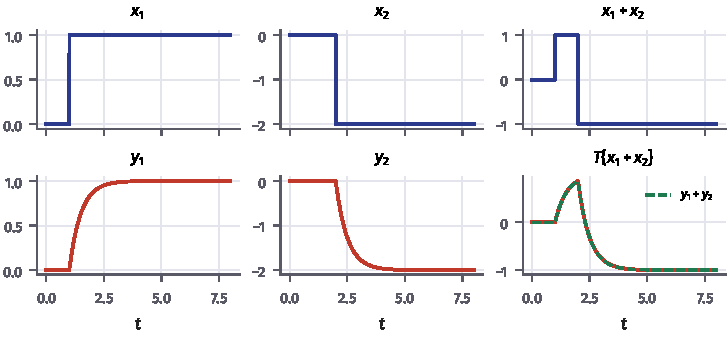
\includegraphics[width=\linewidth]{linealidad}
    \end{column}
  \end{columns}
\end{frame}

\begin{frame}{Invarianza temporal}
  \begin{definicion}[Sistema invariante en el tiempo]
    Un desplazamiento de la entrada produce el mismo desplazamiento de la salida:
    \[
      \T\{x(t)\}=y(t)\ \Rightarrow\ \T\{x(t-t_0)\}=y(t-t_0),\qquad
      \T\{x[n]\}=y[n]\ \Rightarrow\ \T\{x[n-n_0]\}=y[n-n_0]
    \]
  \end{definicion}
  \begin{columns}[c]
    \begin{column}{0.46\textwidth}
      \small
      \alert{Cómo comprobarlo}: calcula la respuesta a $x[n-n_0]$ y compárala con $y[n-n_0]$.
      \smallskip

      Ej.: $y[n]=n\,x[n]$. La respuesta a $x[n-n_0]$ es $n\,x[n-n_0]$, pero $y[n-n_0]=(n-n_0)\,x[n-n_0]$: \alert{no es invariante}.
      \medskip

      \alert{LTI}: lineal e invariante en el tiempo.
    \end{column}
    \begin{column}{0.52\textwidth}
      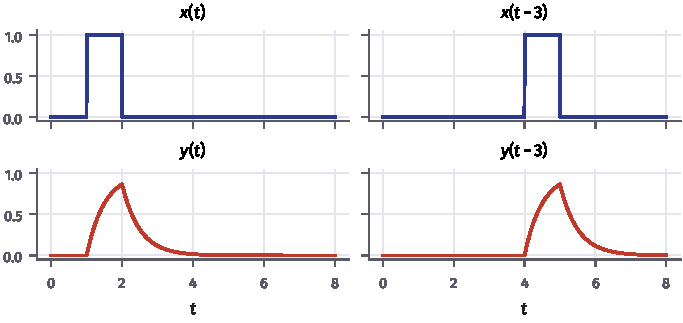
\includegraphics[width=\linewidth]{invarianza}
    \end{column}
  \end{columns}
\end{frame}

\begin{frame}{Ejemplos: ¿qué propiedades cumplen?}
  \begin{center}
    \small
    \renewcommand{\arraystretch}{1.3}
    \begin{tabular}{@{}lcccccc@{}}
      \toprule
      Sistema & Memoria & Causal & Estable & Lineal & Invariante & Invertible\\\midrule
      $y(t)=x^2(t)$ & no & sí & sí & no & sí & no\\
      $y(t)=x(t)+1$ & no & sí & sí & \alert{no} & sí & sí\\
      $y[n]=n\,x[n]$ & no & sí & \alert{no} & sí & \alert{no} & no\\
      $y(t)=x(2t)$ & sí & \alert{no} & sí & sí & \alert{no} & sí\\
      $y[n]=x[n]-x[n-1]$ & sí & sí & sí & sí & sí & no\\
      $y(t)=\int_{-\infty}^{t}x(\tau)\dd\tau$ & sí & sí & \alert{no} & sí & sí & sí\\
      $y[n]=x[-n]$ & sí & no & sí & sí & no & sí\\\bottomrule
    \end{tabular}
  \end{center}
  \begin{itemize}\footnotesize
    \item $y[n]=n\,x[n]$: con $x[n]=1$ (acotada) la salida $y[n]=n$ no está acotada; y $x[0]$ se pierde.
    \item $y(t)=x(2t)$: $y(1)=x(2)$ usa la entrada futura.
    \item $y[n]=x[n]-x[n-1]$: cualquier constante da salida nula, así que no se puede recuperar la entrada.
  \end{itemize}
\end{frame}

\begin{frame}{En código: comprobar la linealidad}
  Probar con señales aleatorias no demuestra la linealidad, pero un solo contraejemplo basta para descartarla.
  \medskip
  \codigo{comprobar_linealidad}
  \herramienta{T1-propiedades-sistemas}
\end{frame}

\begin{frame}{Interconexión de sistemas}
  \begin{columns}[c]
    \begin{column}{0.56\textwidth}
      \centering
      \begin{tikzpicture}[node distance=0.9cm, every node/.style={font=\small}, scale=0.85, transform shape]
        \node (x1) {$x$};
        \node[bloque, right=of x1] (A1) {$\T_1$};
        \node[bloque, right=of A1] (B1) {$\T_2$};
        \node[right=of B1] (y1) {$y$};
        \draw[flecha] (x1) -- (A1); \draw[flecha] (A1) -- (B1); \draw[flecha] (B1) -- (y1);
        \node[above=0.1cm of A1, xshift=0.9cm, pdsgris] {\scriptsize serie (cascada)};
      \end{tikzpicture}\\[2mm]
      \begin{tikzpicture}[node distance=0.6cm and 0.9cm, every node/.style={font=\small}, scale=0.85, transform shape]
        \node (x2) {$x$};
        \coordinate[right=0.5cm of x2] (b);
        \node[bloque, above right=0.15cm and 0.8cm of b] (A2) {$\T_1$};
        \node[bloque, below right=0.15cm and 0.8cm of b] (B2) {$\T_2$};
        \node[sumador, right=2.6cm of b] (s) {$+$};
        \node[right=0.6cm of s] (y2) {$y$};
        \draw[thick, pdsgris] (x2) -- (b);
        \draw[flecha] (b) |- (A2); \draw[flecha] (b) |- (B2);
        \draw[flecha] (A2) -| (s); \draw[flecha] (B2) -| (s); \draw[flecha] (s) -- (y2);
        \node[pdsgris] at ([yshift=0.5cm]A2.north) {\scriptsize paralelo};
      \end{tikzpicture}\\[1mm]
      \begin{tikzpicture}[node distance=0.9cm, every node/.style={font=\small}, scale=0.85, transform shape]
        \node (x3) {$x$};
        \node[sumador, right=0.6cm of x3] (s3) {$+$};
        \node[bloque, right=of s3] (G) {$G$};
        \coordinate[right=0.6cm of G] (c3);
        \node[right=0.5cm of c3] (y3) {$y$};
        \node[bloque, below=0.4cm of G] (Hr) {$K$};
        \draw[flecha] (x3) -- (s3); \draw[flecha] (s3) -- (G); \draw[thick, pdsgris] (G) -- (c3);
        \draw[flecha] (c3) -- (y3);
        \draw[flecha] (c3) |- (Hr); \draw[flecha] (Hr) -| node[pos=0.9, left]{$-$} (s3);
        \node[pdsgris, above=0.05cm of G] {\scriptsize realimentación};
      \end{tikzpicture}
    \end{column}
    \begin{column}{0.42\textwidth}
      Para sistemas LTI:
      \begin{itemize}\small
        \item Serie: $h=h_1\conv h_2$, \ $H=H_1H_2$.\\
          \gris{El orden no importa (conmutativa).}
        \item Paralelo: $h=h_1+h_2$, \ $H=H_1+H_2$.
        \item Realimentación negativa:
          \[H=\frac{G}{1+G\,K}\]
      \end{itemize}
      \nota{$H$ representa la transformada de Laplace, Z o Fourier de $h$.}
    \end{column}
  \end{columns}
\end{frame}

% =====================================================================
\section{Sistemas LTI}

\begin{frame}{Respuesta al impulso y convolución}
  \begin{definicion}[Respuesta al impulso]
    $h(t)=\T\{\delta(t)\}$, \qquad $h[n]=\T\{\delta[n]\}$
  \end{definicion}
  \alert{Deducción en discreto}, a partir de $x[n]=\sum_k x[k]\,\delta[n-k]$:
  \[
    y[n]=\T\Big\{\sum_k x[k]\,\delta[n-k]\Big\}
    \overset{\text{lineal}}{=}\sum_k x[k]\,\T\{\delta[n-k]\}
    \overset{\text{invariante}}{=}\sum_k x[k]\,h[n-k]=(x\conv h)[n]
  \]
  En continuo, igual con $x(t)=\int x(\tau)\,\delta(t-\tau)\dd\tau$:
  \[
    y(t)=\int_{-\infty}^{\infty}x(\tau)\,h(t-\tau)\dd\tau=(x\conv h)(t)
  \]
  \begin{importante}[Consecuencia]
    Un sistema LTI queda \alert{completamente caracterizado} por su respuesta al impulso.
  \end{importante}
\end{frame}

\begin{frame}{Propiedades de un sistema LTI a partir de $h$}
  \begin{center}
    \renewcommand{\arraystretch}{1.45}
    \begin{tabular}{@{}lll@{}}
      \toprule
      Propiedad & Continuo & Discreto\\\midrule
      Sin memoria & $h(t)=K\,\delta(t)$ & $h[n]=K\,\delta[n]$\\
      Causal & $h(t)=0\ \ \forall t<0$ & $h[n]=0\ \ \forall n<0$\\
      Estable (BIBO) & $\displaystyle\int_{-\infty}^{\infty}\abs{h(t)}\dd t<\infty$ & $\displaystyle\sum_{n=-\infty}^{\infty}\abs{h[n]}<\infty$\\
      Invertible & $h\conv h_{\mathrm{inv}}=\delta$ & $h\conv h_{\mathrm{inv}}=\delta$\\\bottomrule
    \end{tabular}
  \end{center}
  \begin{itemize}\small
    \item Estabilidad (suficiencia): si $\abs{x}\le B$, \ $\abs{y[n]}\le\sum_k\abs{h[k]}\,\abs{x[n-k]}\le B\sum_k\abs{h[k]}$.
    \item Respuesta al escalón: $s(t)=\int_{-\infty}^{t}h(\tau)\dd\tau$, \ $s[n]=\sum_{k=-\infty}^{n}h[k]$; y al revés, $h(t)=s'(t)$, $h[n]=s[n]-s[n-1]$.
  \end{itemize}
\end{frame}

\begin{frame}{Exponenciales complejas: autofunciones de los sistemas LTI}
  Con $x(t)=\e^{st}$ ($s\in\C$) y conmutando la convolución:
  \[
    y(t)=\int_{-\infty}^{\infty}h(\tau)\,\e^{s(t-\tau)}\dd\tau
    =\e^{st}\underbrace{\int_{-\infty}^{\infty}h(\tau)\,\e^{-s\tau}\dd\tau}_{H(s)}
    =H(s)\,\e^{st}
  \]
  En discreto, con $x[n]=z^n$: \ $y[n]=H(z)\,z^n$, \ $H(z)=\sum_k h[k]\,z^{-k}$.
  \begin{block}{Respuesta en frecuencia ($s=j\omega$, $z=\e^{j\Omega}$)}
    \begin{itemize}\small
      \item $\e^{j\omega_0t}\ \to\ H(j\omega_0)\,\e^{j\omega_0t}$: misma frecuencia, amplitud por $\abs{H}$, fase desplazada $\arg H$.
      \item Si $h$ es real: $A\cos(\omega_0t+\phi)\ \to\ A\,\abs{H(j\omega_0)}\cos\big(\omega_0t+\phi+\arg H(j\omega_0)\big)$.
      \item Periódica: $x(t)=\sum_kc_k\e^{jk\omega_0t}\ \to\ y(t)=\sum_kc_k\,H(jk\omega_0)\,\e^{jk\omega_0t}$.
      \item General: $Y(j\omega)=H(j\omega)\,\Xc$, \ $Y(\e^{j\Omega})=H(\e^{j\Omega})\,\Xd$.
    \end{itemize}
  \end{block}
  {\footnotesize\color{pdsgris}Si la entrada empieza en $t=0$ y el sistema es estable, dan la respuesta en régimen permanente.}
\end{frame}

% =====================================================================
\section{Sistemas LTI continuos}

\begin{frame}{Ecuación diferencial y función de transferencia}
  Los sistemas LTI continuos de orden finito se describen con una ecuación diferencial lineal de coeficientes constantes:
  \[
    \sum_{k=0}^{N}a_k\,\dvn{y(t)}{t}{k}=\sum_{k=0}^{M}b_k\,\dvn{x(t)}{t}{k}
    \quad\overset{\Lap}{\longrightarrow}\quad
    H(s)=\frac{Y(s)}{X(s)}=\frac{\sum_{k=0}^{M}b_k\,s^k}{\sum_{k=0}^{N}a_k\,s^k}
  \]
  \begin{itemize}
    \item $H(s)=\Lap\{h(t)\}$ es la \alert{función de transferencia}: un cociente de polinomios.
    \item \alert{Ceros}: raíces del numerador. \alert{Polos}: raíces del denominador.
    \item Sistema dinámico si $N\ge1$. Realizable sin derivadores ideales si $M\le N$ (propia).
  \end{itemize}
  \begin{importante}[Estabilidad de un sistema causal]
    Causal y estable $\iff$ todos los polos en el semiplano izquierdo: $\Re\{p_i\}<0$.\\
    {\small Equivale a que la ROC (a la derecha del polo más a la derecha) contenga el eje $j\omega$.}
  \end{importante}
\end{frame}

\begin{frame}{Polos y forma de la respuesta al impulso}
  Cada polo $p$ aporta a $h(t)$ un \alert{modo} $\e^{pt}u(t)$; un par complejo $\sigma\pm j\omega_0$ aporta $\e^{\sigma t}\cos(\omega_0t+\phi)$.
  \begin{center}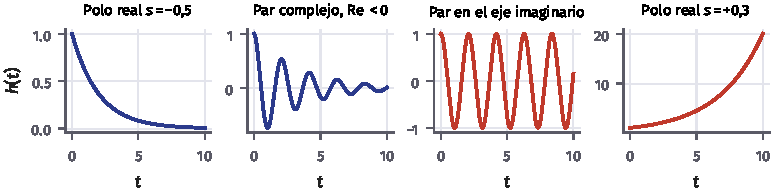
\includegraphics[width=0.95\linewidth]{polos_estabilidad_s}\end{center}
  \begin{itemize}\small
    \item $\Re\{p\}<0$: el modo decae (estable). Cuanto más a la izquierda, más rápido.
    \item $\Re\{p\}=0$: oscilación mantenida (marginalmente estable, \alert{no} BIBO estable: una entrada a esa frecuencia hace crecer la salida sin límite).
    \item $\Re\{p\}>0$: el modo crece (inestable).
  \end{itemize}
\end{frame}

\begin{frame}{Ejemplo: circuito RC}
  \begin{columns}[c]
    \begin{column}{0.5\textwidth}
      $RC\,\dv{y}{t}+y=x$ \quad$\Rightarrow$\quad $H(s)=\dfrac{1}{1+RCs}$
      \begin{itemize}\small
        \item Un polo en $s=-1/RC$: causal y estable.
        \item $h(t)=\frac{1}{RC}\e^{-t/RC}u(t)$
        \item Escalón: $s(t)=\big(1-\e^{-t/RC}\big)u(t)$
        \item $\abs{H(j\omega)}=1/\sqrt{1+(\omega RC)^2}$: paso bajo con frecuencia de corte $\omega_c=1/RC$ ($-3$\,dB).
      \end{itemize}
    \end{column}
    \begin{column}{0.48\textwidth}
      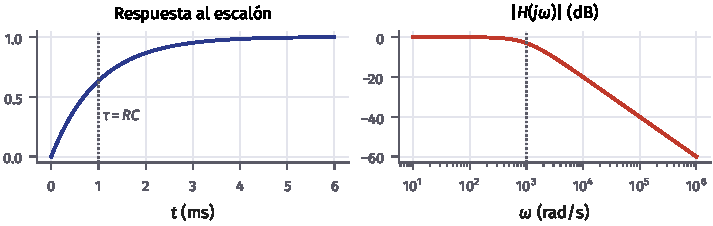
\includegraphics[width=\linewidth]{rc_respuestas}
    \end{column}
  \end{columns}
  \medskip
  \codigo{lti_continuo}
  \herramienta{T1-respuesta-lti-continua}
\end{frame}

% =====================================================================
\section{Sistemas LTI discretos}

\begin{frame}{Ecuación en diferencias y función de transferencia}
  Forma estándar (la que usan \texttt{filter} y \texttt{lfilter}), con $a_0=1$:
  \[
    \sum_{k=0}^{N}a_k\,y[n-k]=\sum_{k=0}^{M}b_k\,x[n-k]
    \quad\overset{\Zt}{\longrightarrow}\quad
    H(z)=\frac{\sum_{k=0}^{M}b_k\,z^{-k}}{1+\sum_{k=1}^{N}a_k\,z^{-k}}
  \]
  \begin{itemize}
    \item Se calcula de forma \alert{recursiva}: $y[n]=\sum_{k=0}^{M}b_k\,x[n-k]-\sum_{k=1}^{N}a_k\,y[n-k]$.
    \item $H(z)=\Zt\{h[n]\}$; polos y ceros, igual que en continuo.
  \end{itemize}
  \begin{importante}[Estabilidad de un sistema causal]
    Causal y estable $\iff$ todos los polos dentro de la circunferencia unidad: $\abs{p_i}<1$.\\
    {\small Equivale a que la ROC ($\abs{z}>\max\abs{p_i}$) contenga la circunferencia unidad.}
  \end{importante}
  \nota{Con adelantos, $\sum a_k y[n+k]=\sum b_k x[n+k]$, se obtiene lo mismo multiplicando numerador y denominador por $z^{-N}$.}
\end{frame}

\begin{frame}{Polos y forma de la respuesta al impulso}
  Cada polo $p$ aporta a $h[n]$ un modo $p^n u[n]$; un par $r\e^{\pm j\Omega_0}$ aporta $r^n\cos(\Omega_0n+\phi)$.
  \begin{center}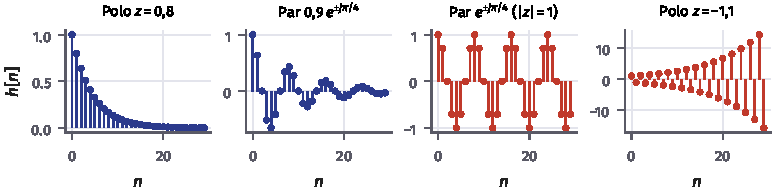
\includegraphics[width=0.95\linewidth]{polos_estabilidad_z}\end{center}
  \begin{itemize}\small
    \item $\abs{p}<1$: decae; $\abs{p}=1$: oscilación mantenida (no BIBO estable); $\abs{p}>1$: crece.
    \item Polo real negativo: la respuesta alterna de signo.
  \end{itemize}
\end{frame}

\begin{frame}{En código: sistema discreto de primer orden}
  \codigo{lti_discreto}
  \nota{Convenio de \texttt{filter}/\texttt{lfilter}: \texttt{b} son los coeficientes de $x[n-k]$ y \texttt{a} los de $y[n-k]$, con \texttt{a[0]=1}.}
  \herramienta{T1-respuesta-lti-discreta}
\end{frame}

\begin{frame}{Sistemas FIR e IIR}
  \begin{columns}[T]
    \begin{column}{0.5\textwidth}
      \alert{FIR} (\emph{finite impulse response})
      \begin{itemize}\small
        \item No recursivo: $a_k=0$ para $k\ge1$.
        \[y[n]=\sum_{k=0}^{M}b_k\,x[n-k]\]
        $h[n]=b_n$ para $0\le n\le M$; $0$ en el resto.
        \item $M+1$ coeficientes; polos en $z=0$.
        \item \alert{Siempre estable}; puede tener fase lineal.
      \end{itemize}
    \end{column}
    \begin{column}{0.48\textwidth}
      \alert{IIR} (\emph{infinite impulse response})
      \begin{itemize}\small
        \item Recursivo: algún $a_k\neq0$ con $k\ge1$.
        \item $h[n]$ de duración infinita.
        \item Puede ser inestable: hay que comprobar los polos.
        \item Menos coeficientes que un FIR para la misma selectividad.
      \end{itemize}
    \end{column}
  \end{columns}
  \begin{columns}[c]
    \begin{column}{0.44\textwidth}
      \small
      Media móvil (FIR): $y[n]=\frac15\sum_{k=0}^{4}x[n-k]$\\[1mm]
      Suavizado exponencial (IIR):\\ $y[n]=0{,}8\,y[n-1]+0{,}2\,x[n]$
    \end{column}
    \begin{column}{0.54\textwidth}
      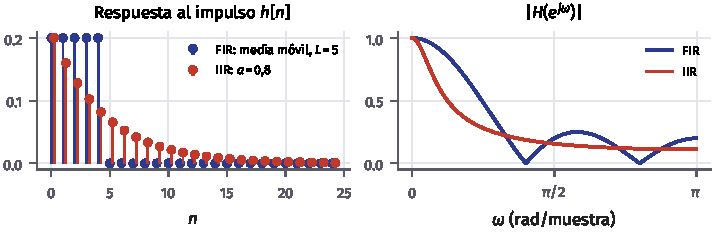
\includegraphics[width=0.9\linewidth]{fir_iir}
    \end{column}
  \end{columns}
\end{frame}

\begin{frame}{Diagramas de bloques}
  \begin{columns}[c]
    \begin{column}{0.52\textwidth}
      \centering
      \alert{FIR} (línea de retardos)\\[2mm]
      \begin{tikzpicture}[every node/.style={font=\small}]
        \node (x) at (0,0) {$x[n]$};
        \node[bloque, minimum width=9mm] (d1) at (2,0) {$z^{-1}$};
        \node[bloque, minimum width=9mm] (d2) at (4,0) {$z^{-1}$};
        \node[sumador] (s1) at (3,-1.6) {$+$};
        \node[sumador] (s2) at (5,-1.6) {$+$};
        \draw[flecha] (x) -- (d1); \draw[flecha] (d1) -- (d2);
        \draw[thick, pdsgris] (d2) -- (5,0);
        \draw[flecha] (1,0) -- node[left]{$b_0$} (1,-1.6) -- (s1);
        \draw[flecha] (3,0) -- node[right]{$b_1$} (s1);
        \draw[flecha] (5,0) -- node[right]{$b_2$} (s2);
        \draw[flecha] (s1) -- (s2);
        \draw[flecha] (s2) -- (6.2,-1.6) node[right]{$y[n]$};
        \fill[pdsgris] (1,0) circle (1.2pt) (3,0) circle (1.2pt);
      \end{tikzpicture}\\[1mm]
      {\small $y[n]=b_0x[n]+b_1x[n-1]+b_2x[n-2]$}
    \end{column}
    \begin{column}{0.46\textwidth}
      \centering
      \alert{IIR de primer orden}\\[2mm]
      \begin{tikzpicture}[node distance=0.6cm and 0.8cm, every node/.style={font=\small}]
        \node (x) {$x[n]$};
        \node[bloque, minimum width=9mm, right=of x] (b0) {$b_0$};
        \node[sumador, right=of b0] (s) {$+$};
        \coordinate[right=0.8cm of s] (c);
        \node[right=0.4cm of c] (y) {$y[n]$};
        \node[bloque, minimum width=9mm, below=0.6cm of c] (d) {$z^{-1}$};
        \node[bloque, minimum width=9mm, left=0.5cm of d] (a1) {$-a_1$};
        \draw[flecha] (x) -- (b0); \draw[flecha] (b0) -- (s); \draw[thick, pdsgris] (s) -- (c);
        \draw[flecha] (c) -- (y);
        \draw[flecha] (c) -- (d); \draw[flecha] (d) -- (a1); \draw[flecha] (a1) -| (s);
      \end{tikzpicture}\\[2mm]
      {\small $y[n]=b_0\,x[n]-a_1\,y[n-1]$}
    \end{column}
  \end{columns}
  \bigskip
  {\small Con sumadores, multiplicadores y retardos $z^{-1}$ se implementa cualquier ecuación en diferencias: es lo que ejecuta un DSP o un microcontrolador.}
\end{frame}

\begin{frame}{¿Hay sistemas FIR en tiempo continuo?}
  \begin{itemize}
    \item Un sistema continuo descrito por una ecuación diferencial de orden finito tiene $H(s)$ racional, y su $h(t)$ es una suma de modos $\e^{p_it}$: \alert{siempre de duración infinita} (salvo términos $\delta$ si $M\ge N$).
    \item Existen sistemas continuos con $h(t)$ de duración finita, como el integrador de ventana
      \[
        y(t)=\int_{t-T}^{t}x(\tau)\dd\tau,\qquad h(t)=u(t)-u(t-T),\qquad H(s)=\frac{1-\e^{-sT}}{s},
      \]
      pero su $H(s)$ \alert{no es racional}: no se construyen con un número finito de componentes R, L, C.
    \item En discreto, en cambio, un FIR es trivial de implementar: basta una línea de retardos.
  \end{itemize}
  \nota{Esta es una de las ventajas del procesado digital: los FIR (fase lineal, siempre estables) solo son prácticos en discreto.}
\end{frame}

% =====================================================================
\section*{Resumen}
\begin{frame}{Conceptos importantes}
  \begin{columns}[T]
    \begin{column}{0.5\textwidth}
      \begin{itemize}
        \item Propiedades: memoria, causalidad, estabilidad BIBO, invertibilidad, \alert{linealidad} e \alert{invarianza temporal}.
        \item Un sistema LTI queda caracterizado por $h$: $y=x\conv h$.
        \item Causalidad y estabilidad se leen en $h$ y en los polos.
      \end{itemize}
    \end{column}
    \begin{column}{0.5\textwidth}
      \begin{itemize}
        \item Las exponenciales son autofunciones: $\e^{j\omega t}\to H(j\omega)\e^{j\omega t}$.
        \item Cálculo de la respuesta: convolución, Laplace/Z o Fourier.
        \item FIR frente a IIR en sistemas discretos.
      \end{itemize}
    \end{column}
  \end{columns}
  \bigskip
  \gris{Apuntes del Tema 1, secciones 7–9 · Hoja de ejercicios, ejercicios 10–16.}
\end{frame}

\end{document}
